\documentclass[11pt]{article}
\usepackage{graphicx}
\usepackage{tikz}
\usepackage{tikz-qtree}
\usepackage{listings}
\usepackage{mathtools}
\title{ELEC4320 Homework 3}
\author{Dhesant Nakka | 20146587}

\lstset {
  language=C++,
  basicstyle=\footnotesize
}

\newcommand{\textunderscript}[1]{$_{\text{#1}}$}

\begin{document}
\maketitle

\section*{Question 1}
a)
  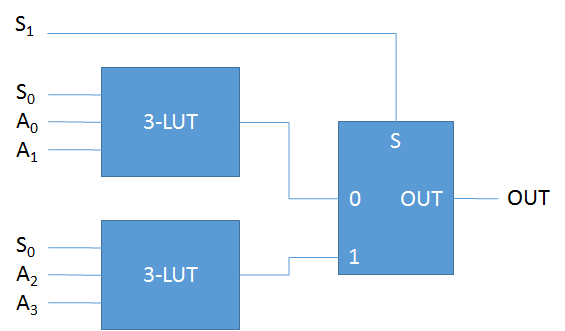
\includegraphics[width=\linewidth]{q1_mux.png}

b)\\*
  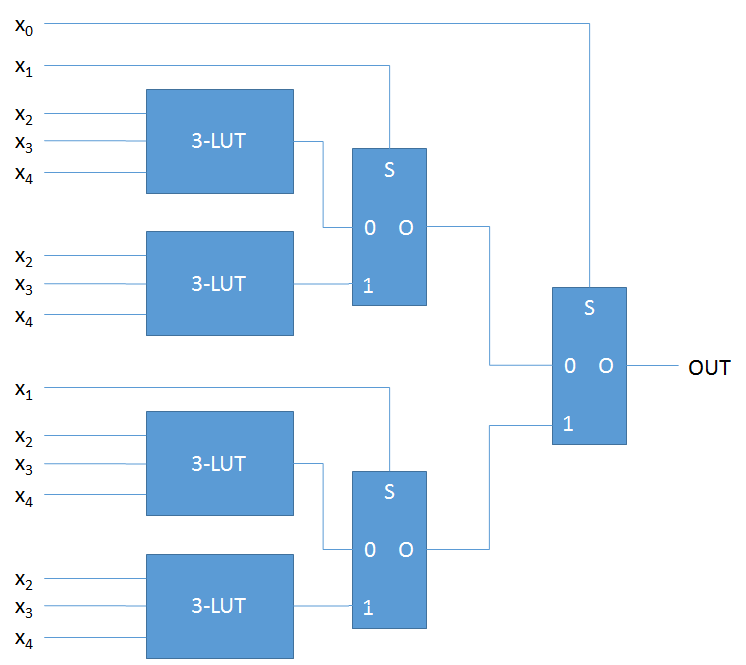
\includegraphics[width=\linewidth]{q1_lut.png}\\\\
  2-input MUX's are created using a 3-LUT that use the following truth table.\\\\
  \begin{tabular}{ | c c c | c | }
    \hline
    S & A & B & O \\
    \hline
    0 & 0 & 0 & 0 \\
    0 & 0 & 1 & 1 \\
    0 & 1 & 0 & 0 \\
    0 & 1 & 1 & 1 \\
    1 & 0 & 0 & 0 \\
    1 & 0 & 1 & 0 \\
    1 & 1 & 0 & 1 \\
    1 & 1 & 1 & 1 \\
    \hline
  \end{tabular}
\section*{Question 2}
System Generator schematic diagram:\\*
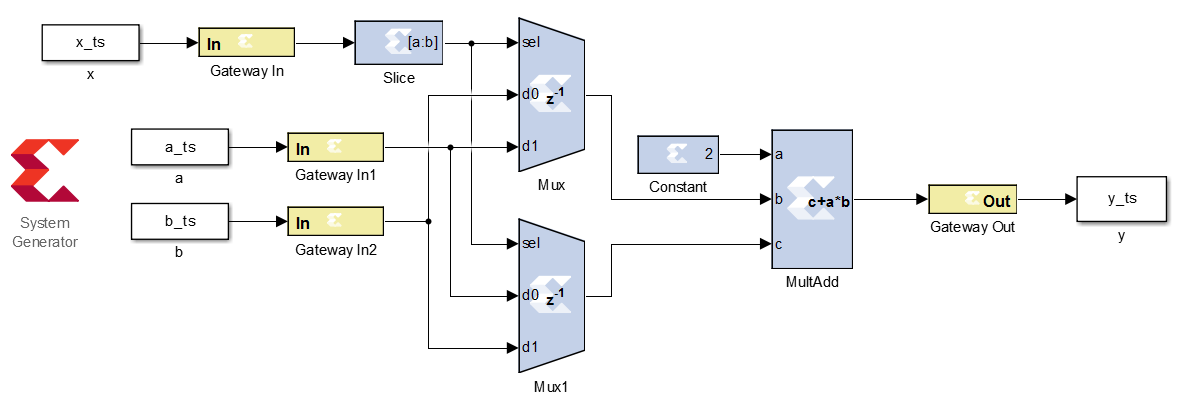
\includegraphics[width=\linewidth]{q2/model.png}\\
Simulink simulation results:\\*
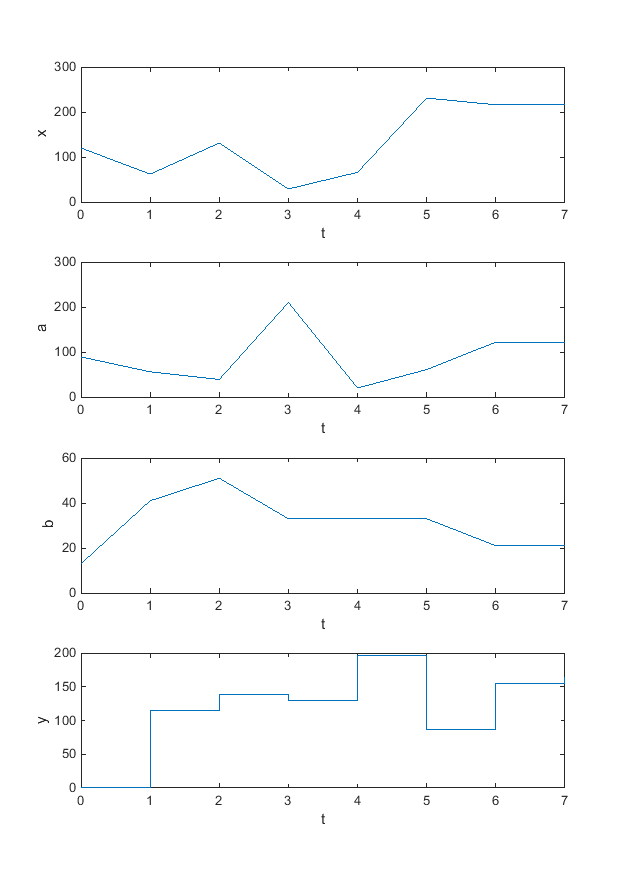
\includegraphics[width=\linewidth]{q2/data_plot.png}

\section*{Question 3}
a)
i)
The longest operation is the two compound adders A1 and A2 in C-step1, requiring a total time of 6 ns. Therefore, the required clock period should be 6ns.\\*

Moving the A2 adder block from C-step1 to C-step2 would satisify the new clock period of 4ns, since the output of A2 is not needed until C-step3 (see Figure \ref{fig:q3_design});

\begin{figure}[h!]
  \centering
  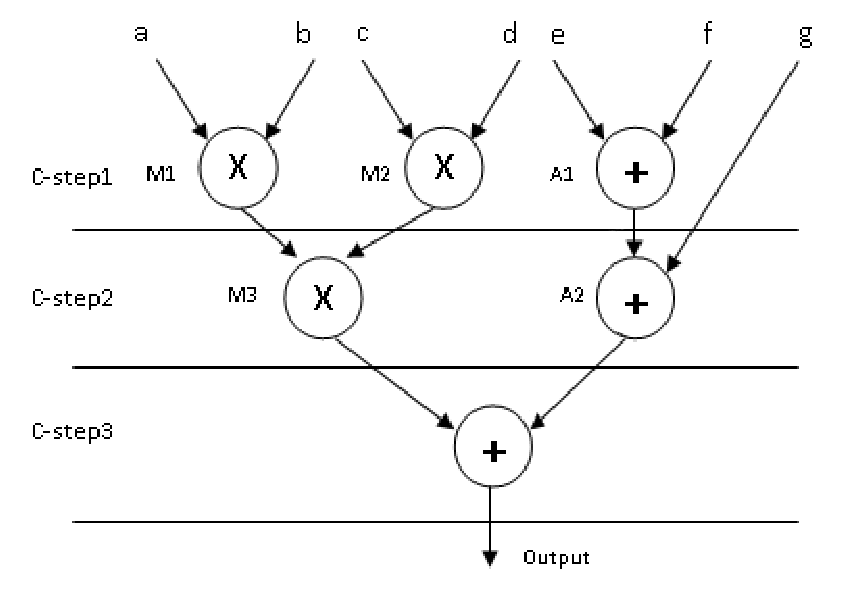
\includegraphics[width=0.8\linewidth]{q3_design.png}
  \caption{The new design schematic to meet the 4ns clock period requirement}
  \label{fig:q3_design}
\end{figure}

ii)
According to the new design, in addition the 2 multipliers and 1 adder needed to implement the design, the design will also need 4 multiplexers to control which input goes to the multiplier and adder blocks, and 3 registers (as seen in Figure \ref{fig:q3_hw}), to store the output from each of the multiplier and adder blocks between each cycle. The assignment can be seen in Figure \ref{fig:q3_assign}. The final schedule can be seen in Table \ref{tab:q3_schedule}. The final hardware diagram can be seen in Figure \ref{fig:q3_hw}.

\begin{figure}[h!]
  \centering
  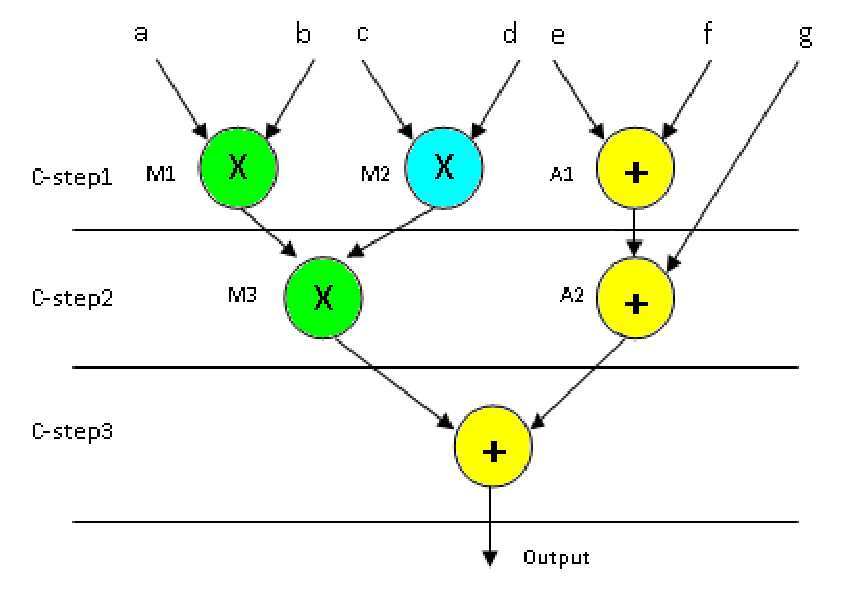
\includegraphics[width=0.8\linewidth]{q3_design2.png}
  \caption{Assignment of the operations to different hardware block}
  \label{fig:q3_assign}
\end{figure}

\begin{table}[h!]
  \centering
  \begin{tabular}{| r | c c c |}
    \hline
    Step & Mult 1 & Mult 2 & Add 1 \\
    \hline
    C-step1 & A $\times$ B & C $\times$ D & E + F \\
    C-step2 & Mult 1 $\times$ Mult 2 & & G + Add 1 \\
    C-step3 & & & Mult 1 + Add 1 \\
    \hline
  \end{tabular}
  \caption{Scheduling of block operations}
  \label{tab:q3_schedule}
\end{table}

\begin{figure}[h!]
  \centering
  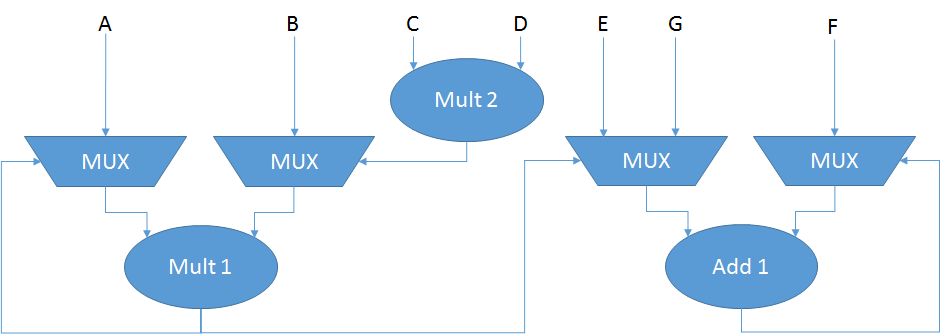
\includegraphics[width=\linewidth]{q3_diagram.png}
  \caption{Block overview of the final implementation}
  \label{fig:q3_hw}
\end{figure}

\clearpage

b)
\begin{lstlisting}[showstringspaces=false]
#include "ap_cin.h"

typedef uint4 t_data4;
typedef uint5 t_data5;
typedef uint8 t_data8;

t_data5 A[10];
t_data8 B[10], C[10];
t_data4 i;

for (i = 0; i < 10; ++i) {
  C[i] = A[i] + B[i];
}
\end{lstlisting}

The new code uses less area because of the reduced width of all the integers. Instead of having to create a 32-bit adder on the FPGA, which will require a lot of LUT's, all that is needed now is at 8-bit LUT adder, since the output value will never exceeed the 8-bit limit of 255. Also, the comparator needed to check the flow of the loop can be made smaller, since it is now a 4-bit integer instead of a 32-bit integer. In addition, since the arrays are also a lot smaller, they use less memory space than before, allowing them to be reshaped to fit into less memory.

\end{document}